\section{Introduction}
\label{sec:intro}
Gamma-ray astronomy is a rather young field of research.
By detecting and reconstructing arrival direction, time and energy
of primary cosmic gamma-rays
The gamma-ray sky is either observed by ground based instruments

, driven by experiments with proprietary software often based
on ROOT, because of the particle physics background. Such 
as HESS, Veritas or Magic.

The Cherenkov Telescope Array will be operated as an open
observatory for the first time. Thus there is a need for
open analysis software as well.

Once the primary photons are reconstructed the format of the data
of all Gamma-ray instrumets can be brought into a common format.
An effort is the gamma-astro data formats \cite{gadf-zenodo}.
The data format is based on FITS  \citep{fits}.


In recent years Python \footnote{\PythonUrl} has established as one of the
standard programming  languages for astronomy \footnote{Citation missing}
as well as data sciences in  general \footnote{Citation missing}.
The success is mostly attributed to the simple and easy to learn syntax,
the ability to act as a "glue" language between different libraries,
the rich eco-system of packages and the open and active (online) community.

Astronomical data analysis software written in Python existed since 2000.
e.g. sherpa \citep{sherpa-2011, sherpa-2009}, or for gamma-ray even
PyFACT \citep{pyfact}.

The short-term success of Pythion lead to a prolifaration of packages, until
\astropy \citep{astropy} was created in 2012. Astropy is and


Gammapy is a Python package for gamma-ray astronomy.

% TODO: describe Context

% TODO: describe goals

TODO: Figure 1: Data -> Gammapy -> Spectra etc with some details 

Basic idea: build on Numpy and Astropy, use Python stack

TODO: Figure 2: Gammapy software stack

Here's a list of references I'd like to cite ... to be incorporated into the
main text somewhere:

\begin{itemize}
\item Gammapy webpage\footnote{\GammapyUrl}
\item Naima\footnote{\NaimaUrl} \citep{Naima}
\item Gammapy use in science publications: \citep{Owen2015}, SNR shell, HGPS
\end{itemize}

* Gammapy – A Python package for gamma-ray astronomy
* Gammapy – A prototype for the CTA science tools 
* Astropy: A community Python package for astronomy
* THE ASTROPY PROJECT: BUILDING AN INCLUSIVE, OPEN-SCIENCE PROJECT AND STATUS OF THE V2.0 CORE PACKAGE
* GammaLib and ctools
* Fermipy proceedings
* SunPy: Python for Solar Physics. An implementation for local correlation tracking
*

\begin{figure}[t]
\centering
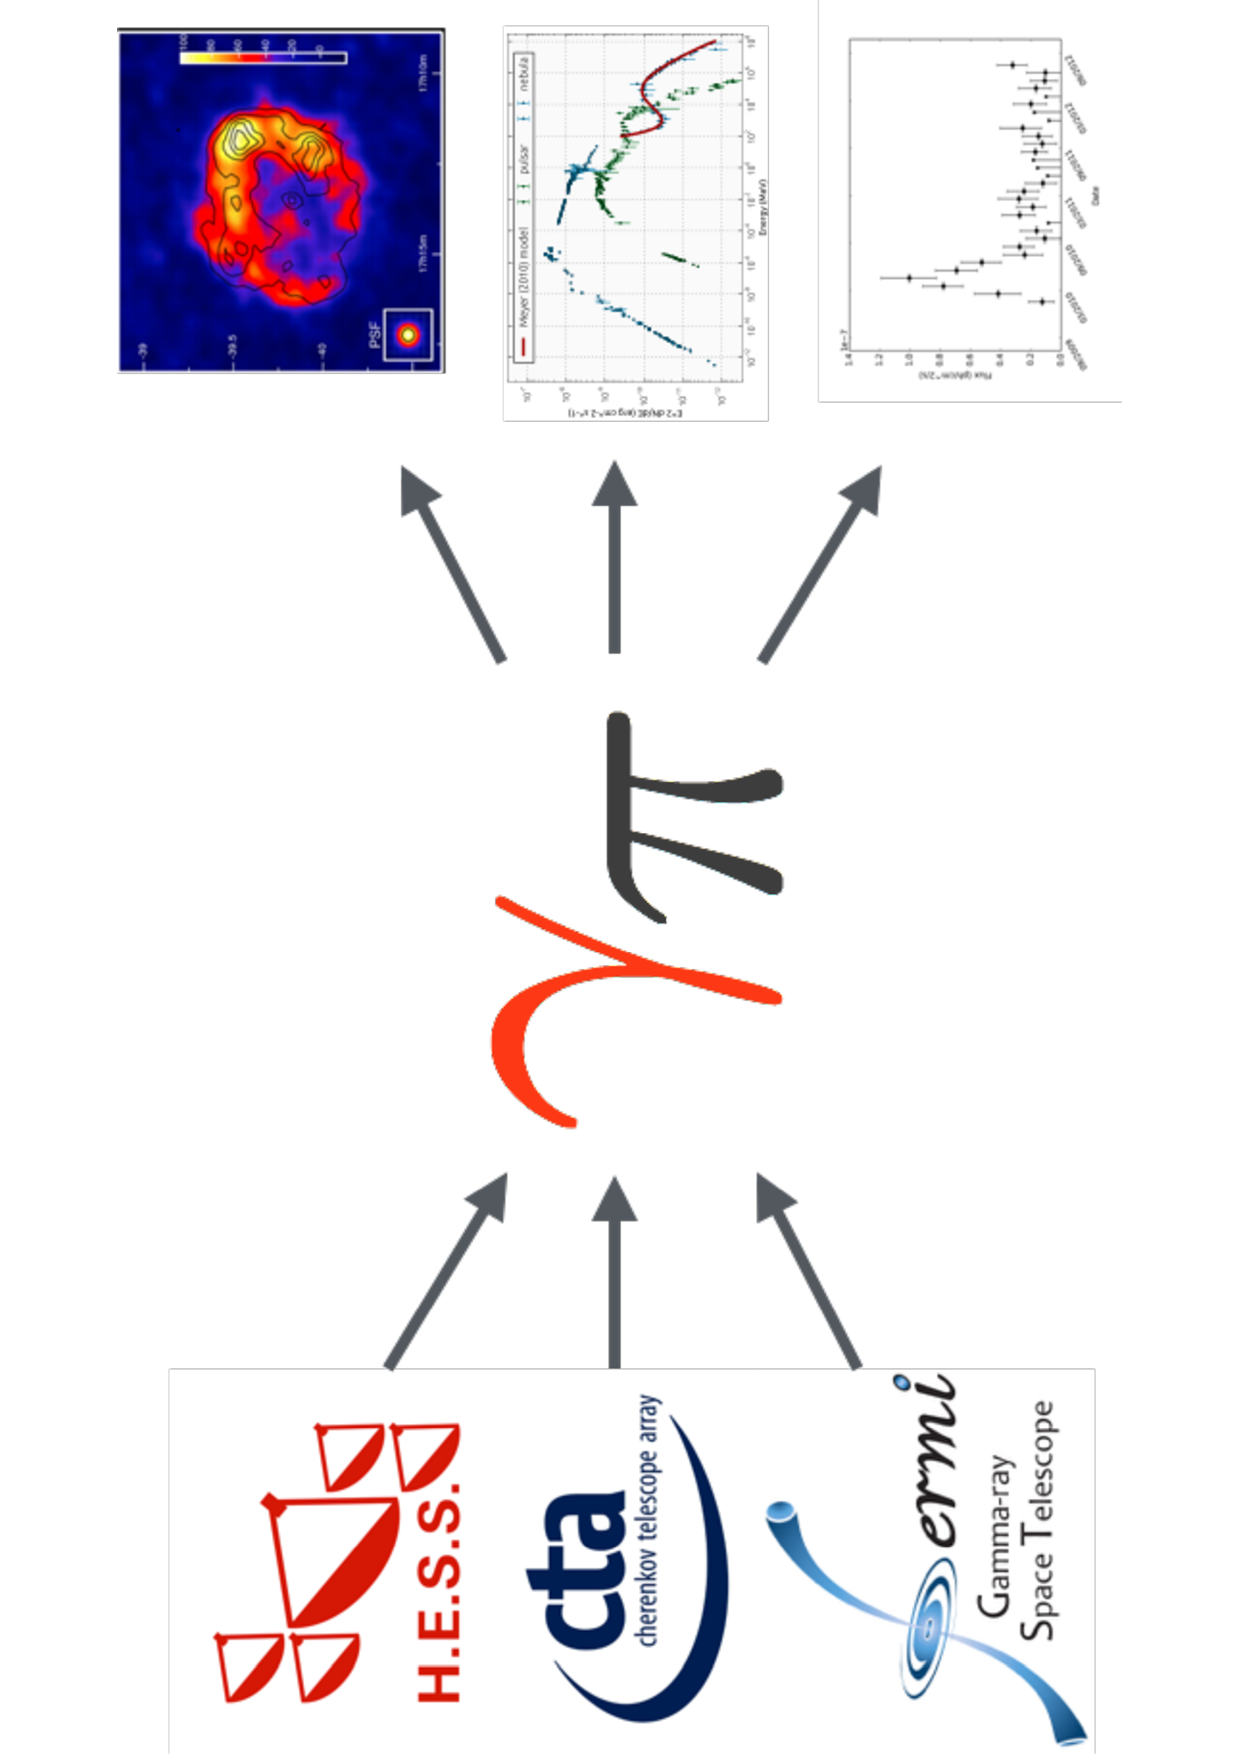
\includegraphics[height=0.5\textwidth, angle=270]{figures/gammapy-big-picture}
\caption{
Gammapy is a Python package for high-level gamma-ray data analysis. Using event
lists, exposures and point spread functions as input you can use it to generate
science results such as images, spectra, light curves or source catalogs. So far
it has been used to simulate and analyse H.E.S.S., CTA and \textit{Fermi}-LAT
data, hopefully it will also be applied to e.g. VERITAS, MAGIC or HAWC data in
the future.
}
\label{fig:big-picture}
\end{figure}

\begin{figure}[t]
\centering
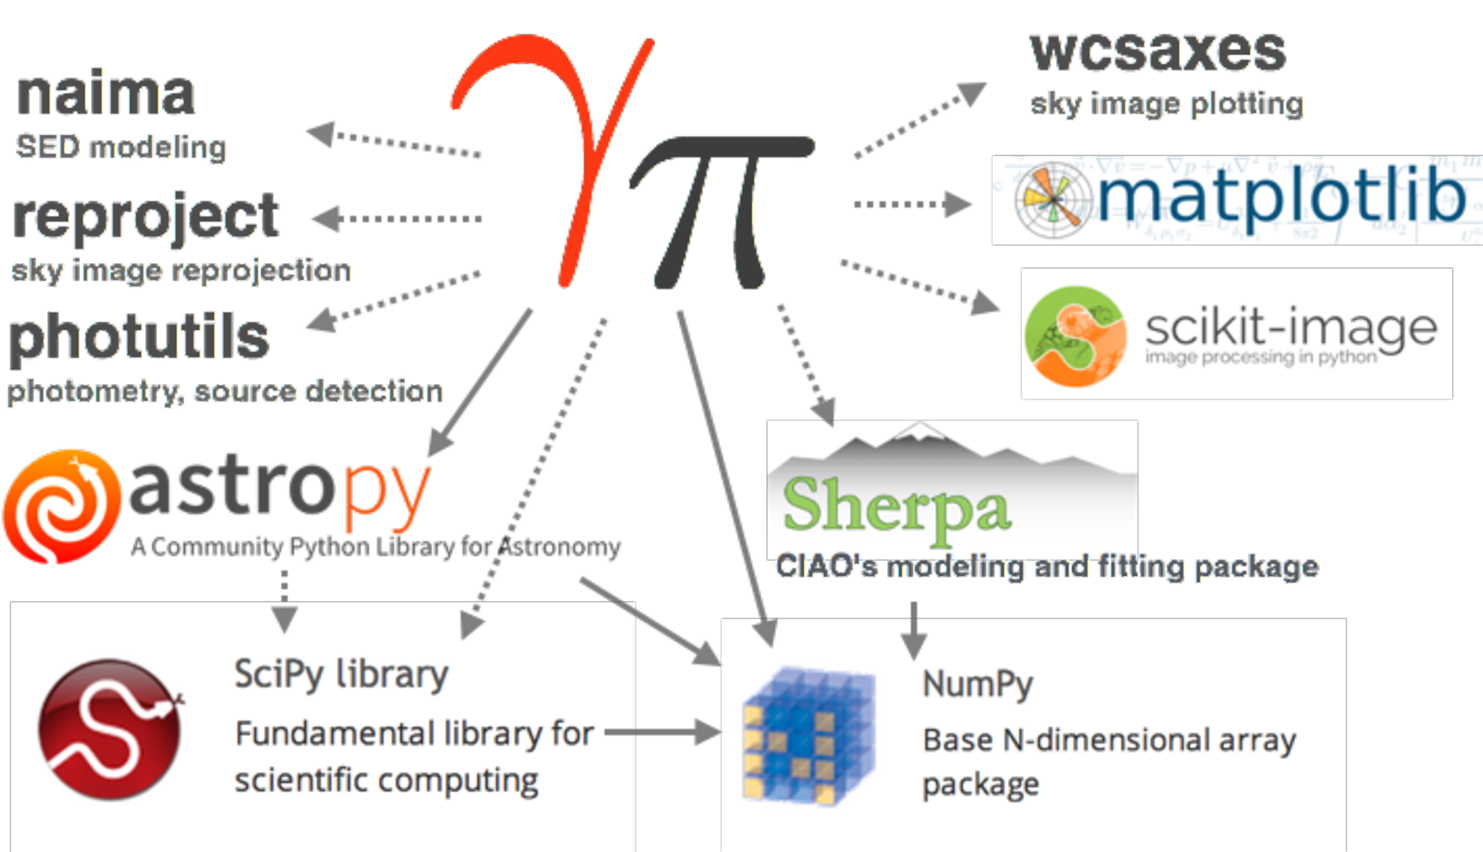
\includegraphics[width=0.5\textwidth]{figures/gammapy-dependencies}
\caption{
The Gammapy stack. Required dependencies Numpy and Astropy are illustrated with
solid arrows, optional dependencies (the rest) with dashed arrows.
}
\label{fig:dependencies}
\end{figure}
